%%%%%%%%%%%%%%%%%%%% Chapter 1
\chapter{Introduction} % Main chapter title
\label{Chapter1} % For referencing the chapter elsewhere, use
%----------------------------------------------------------------------------------------


\begin{chaptersummary}
This chapter motivates the study by describing scenarios where rigid-link manipulators are limited (narrow workspaces, fragile or irregular objects, and applications that require low distal inertia). It states the central research question: how can tendon-driven mechanisms be designed to provide adaptive, dexterous, and reliable manipulation under these constraints.

The chapter also outlines the thesis structure and main contributions: (1) a mechanism-level study of tension management and proximal actuation; (2) Lasso Gripper as the primary novel mechanism platform, including its concept, prototype, modeling, and qualitative demonstrations; (3) a complementary application case in the form of a handheld motorized laparoscopic instrument developed under the same tendon-driven mechanism framework; and (4) recommendations and future directions for evaluation and clinical translation.
\end{chaptersummary}

% Define some commands to keep the formatting separated from the content
% \newcommand{\keyword}[1]{\textbf{#1}}
% \newcommand{\tabhead}[1]{\textbf{#1}}
% \newcommand{\code}[1]{\texttt{#1}}
% \newcommand{\file}[1]{\texttt{\bfseries#1}}
% \newcommand{\option}[1]{\texttt{\itshape#1}}
\begin{sloppypar}
Robotic manipulation increasingly occurs in constrained environments, including narrow workspaces, fragile or irregular objects, and tasks that require low distal inertia. Rigid-link mechanisms often perform poorly under these conditions. Tendon- and cable-driven systems are attractive because they transmit force through lightweight tensile elements, allow motors to be placed proximally, and provide compliance at contact points. However, such systems introduce engineering challenges including slack accumulation, hysteresis, friction losses, coupling between degrees of freedom, and reduced predictability under varying loads.
\end{sloppypar}

This thesis adopts a mechanism-centered perspective to address these issues. The central question is how tendon-driven mechanisms can be designed to deliver adaptive, dexterous, and reliable manipulation while meeting constraints on size, weight, and compliance. To answer this, the thesis studies two systems under a shared tendon-driven mechanism framework: Lasso Gripper, which is the primary novel mechanism platform and adaptive loop-based end-effector, and a handheld motorized laparoscopic instrument, which serves as a complementary application case focused on guided cable transmission, packaging, and control.

The first embodiment, termed Lasso Gripper, studies how a flexible tensile element can function not only as a transmission component but also as the primary structure for grasp formation. Inspired by traditional capture tools such as the cowboy lasso and the Mongolian Uurga, shown in Fig.\ref{fig:11} and Fig.\ref{fig:12}, the proposed mechanism launches and retracts a controllable string loop to create a large adaptive capture region around the target. This approach differs fundamentally from conventional antipodal grippers, which apply concentrated contact forces over limited areas and often struggle with large, soft, or irregularly shaped objects. By contrast, the string loop enables distributed contact, greater tolerance to positional uncertainty, and a favorable balance between grasp adaptivity and force transmission.
\begin{figure}[htbp]
    \centering
    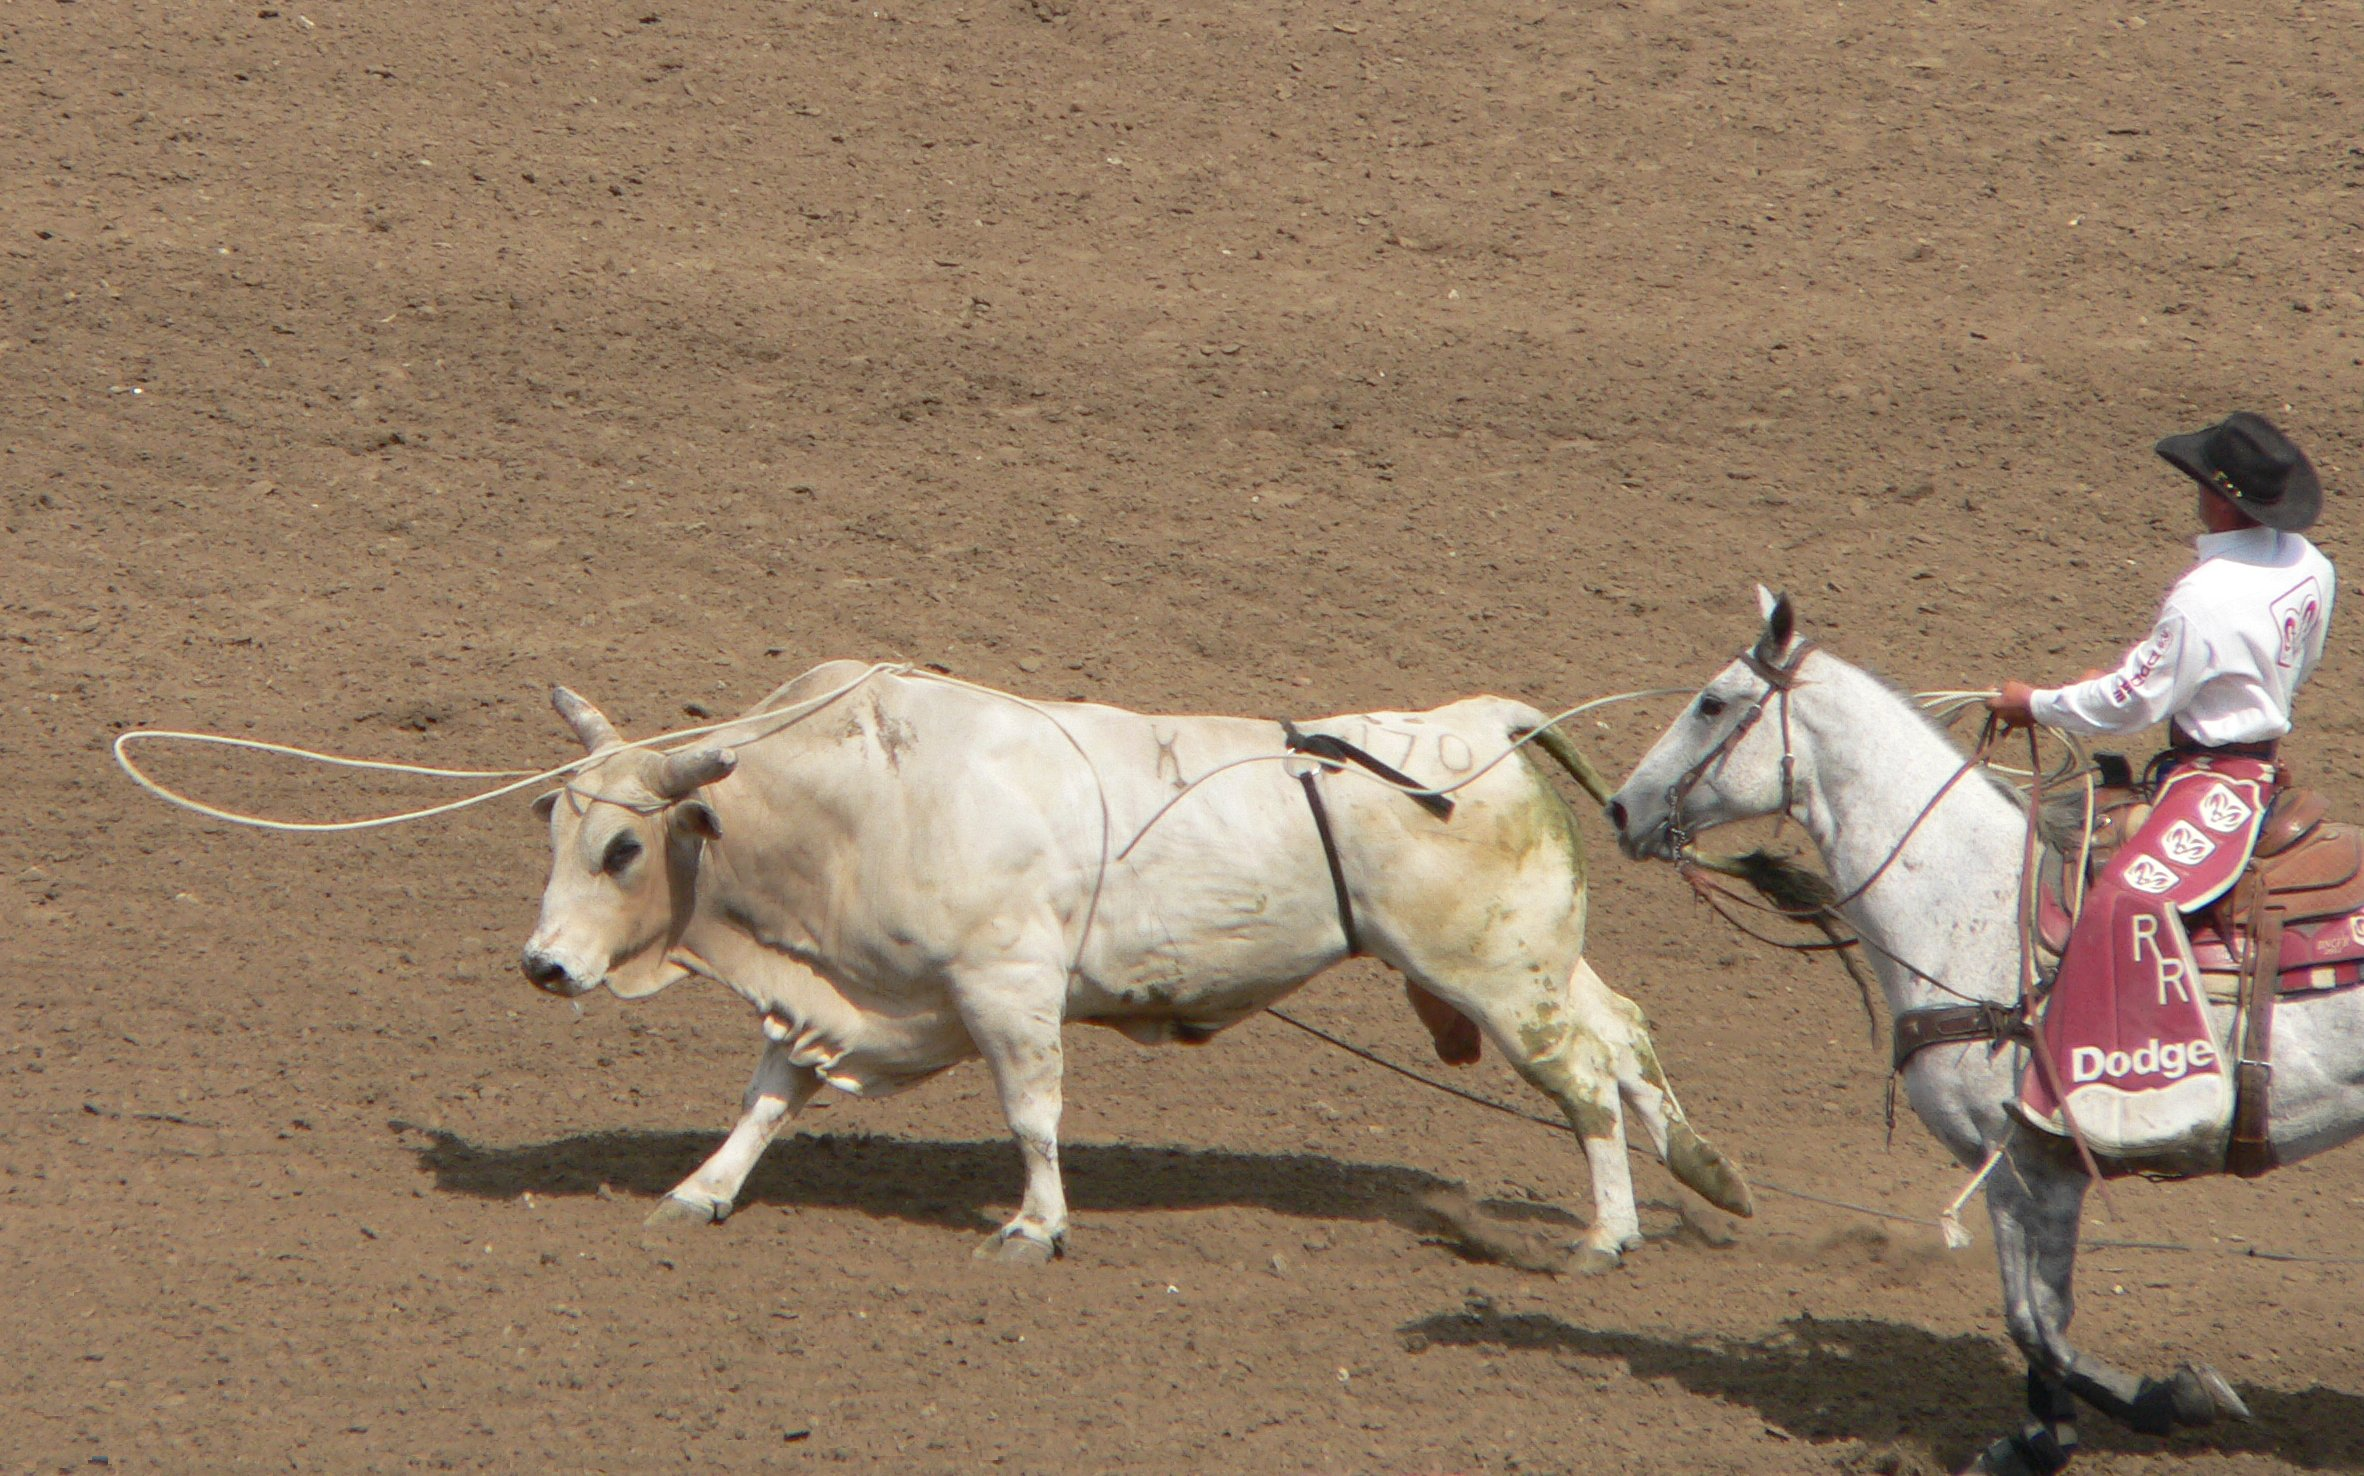
\includegraphics[width=0.7 \linewidth]{Figures/California_rodeo_Salinas_lasso_bull_p1050544.jpg}
    \caption{Traditional cowboy lasso.}
    \label{fig:11}
\end{figure}
\begin{figure}[htbp]
    \centering
    
\includegraphics[width=0.7 \linewidth]{Figures/uurga.jpg}
    \caption{Traditional Mongolian uurga.}
    \label{fig:12}
\end{figure}

\begin{figure}[htbp]
\centering
\begin{tabular}{cc}
\begin{minipage}[t]{0.9\textwidth}
\centering
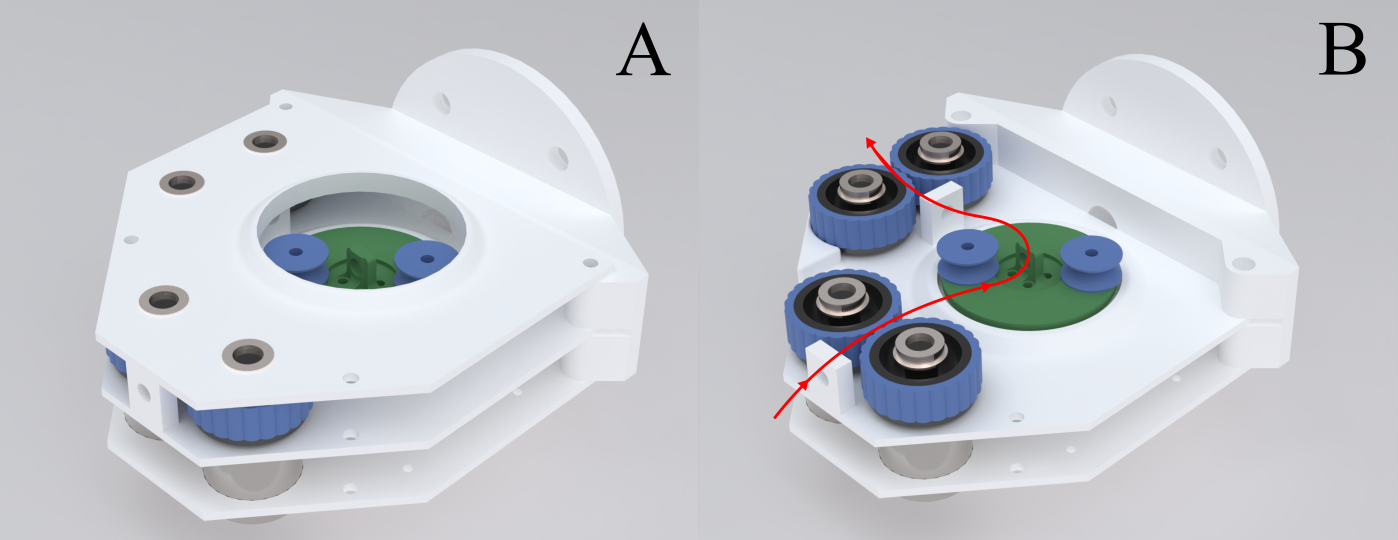
\includegraphics[width=\linewidth]{Figures/Figure1.png}
\caption{Prototype of Lasso Gripper.}
\label{fig:prototype_lasso_gripper}
\end{minipage}
\end{tabular}
\end{figure}

Within this thesis, Lasso Gripper serves as the main mechanism innovation and the central experimental platform. Its development makes it possible to study several mechanism-level questions: how tension can be maintained during reversible actuation, how launch-and-retraction dynamics affect capture range, how a flexible loop can improve robustness to object uncertainty, and how remote actuation can be coordinated to preserve low distal complexity. These questions define the main exploratory contribution of the thesis.

The handheld laparoscopic instrument examines the same tendon-driven variables in a much more constrained application domain. In laparoscopic surgery, surgeons manipulate long and slender tools through small incisions, which severely restrict distal dexterity and attenuate direct haptic perception, as illustrated in Fig.\ref{fig:13}. Conventional instruments typically provide only basic grasping and rotation, while more advanced articulated systems must balance dexterity against weight, complexity, and controllability. Tendon-driven actuation is highly relevant in this context because it permits motors to remain proximal while producing multiple distal degrees of freedom. However, the medical setting imposes additional constraints on size, ergonomic balance, repeatability, safety, and motion fidelity.
\begin{figure}[htbp]
    \centering
    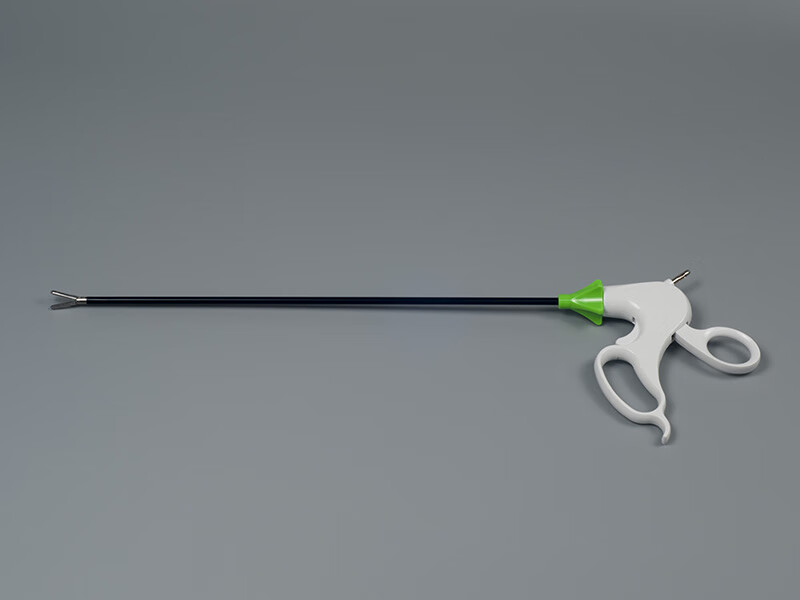
\includegraphics[width=0.7 \linewidth]{Figures/surgical instrument.jpg}
    \caption{Typical single-hole surgical instruments with limited distal dexterity.}
    \label{fig:13}
\end{figure}

The handheld laparoscopic instrument is therefore framed as a complementary application case within the same tendon-driven mechanism framework. It is not treated as a derivative of Lasso Gripper. Instead, it shows how related mechanism variables, including proximal actuation, differential tendon routing, explicit tension management, and sensor-supported control, can be organized in a compact handheld system under practical clinical constraints. This positioning keeps Lasso Gripper as the main innovative platform while allowing the thesis to examine tendon-driven design in a second, application-oriented setting.

The main contributions of this thesis are summarized as follows:
\begin{enumerate}
    \item A mechanism-level study of tendon-driven robotic systems focused on tension management, proximal actuation, compliant interaction, and low distal inertia.
    \item The design, fabrication, and experimental validation of Lasso Gripper as a novel tendon-driven mechanism for adaptive robotic grasping.
    \item The design and implementation of a handheld motorized laparoscopic instrument as a complementary application-oriented tendon-driven system for minimally invasive manipulation.
    \item A unified thesis narrative showing how tendon-driven mechanism principles can be organized across a primary adaptive grasping platform and a secondary medical-device application case.
\end{enumerate}

The remainder of this thesis is organized to follow that mechanism-centered narrative. Chapter 2 reviews related work in laparoscopic end-effectors and adaptive grasping systems, with emphasis on actuation, sensing, and tendon-driven design trade-offs. The subsequent chapters present Lasso Gripper as the primary contribution, including its mechanism design, grasping strategy, dynamic behavior, and experimental validation. The thesis then presents the handheld surgical instrument as a complementary application case under the same tendon-driven framework, focusing on compact device architecture, cable routing design, sensing strategy, and control implementation. The final chapters discuss the broader implications of these results and outline future directions for tendon-driven robotic mechanisms.

\let\cleardoublepage\clearpage
